\documentclass{llncs}
\usepackage[utf8]{inputenc}
\usepackage{epstopdf}
\usepackage{times}
\usepackage{natbib}
\usepackage{amsmath}
\usepackage{dcolumn}
\usepackage{graphicx}
\usepackage{xspace}
\usepackage{color}
\usepackage{listings}
\usepackage{float}
%\usepackage{amsmath, amsthm, amssymb, amsfonts}
%\usepackage{tabularx}
\usepackage{array}
%\usepackage{tabulary}%can use align in tables with line breaks
\usepackage{multirow}
\usepackage{rotating,makecell}
\usepackage{booktabs} %adds new commands toprule midrule and bottomrule for professionally looking tables

\usepackage[breaklinks=true, bookmarksopen=true,bookmarksnumbered=true]{hyperref}
\urlstyle{same}
% \usepackage{titling} % To modify the title
%\usepackage[hmargin=1.3in]{geometry}
% \setlength{\droptitle}{-5em}   % This is your set screw

\usepackage{footnote}


\definecolor{Brown}{cmyk}{0,0.81,1,0.60}
\definecolor{OliveGreen}{cmyk}{0.64,0,0.95,0.40}
\definecolor{CadetBlue}{cmyk}{0.62,0.57,0.23,0}
\definecolor{lightlightgray}{gray}{0.9}

% listing styles
\lstset{
    numberbychapter=false,
    basicstyle=\ttfamily\footnotesize,
    numbers=none,
    captionpos=b,
    frame=single,
    breaklines=true,
    breakatwhitespace,
    columns=fullflexible,
    commentstyle=\itshape\color{OliveGreen},
    keywordstyle=\bfseries\color{CadetBlue}
}


\lstdefinestyle{SPARQL}{
  backgroundcolor=\color{lightlightgray}, % Choose background color
  morecomment=[l]{\#},
  morekeywords={SELECT, CONSTRUCT, FROM, WHERE, FILTER, GROUP BY, IN, AS,
    LIMIT,OFFSET,PREFIX,OPTIONAL,UNION,NOT,EXISTS,AVG,BIND,
    obs,foaf,rdf,skos,rdfs,ex,xsd,owl,skosxl,doap,void,dbo,earl,cex,qb}
 }

\lstdefinestyle{Turtle}{
  backgroundcolor=\color{lightlightgray}, % Choose background color
  morecomment=[l]{\#},
  morekeywords={@PREFIX,BASE,a,foaf, @prefix, rdf,
    obs,qb,cex,skos, skosxl, rdf, rdfs, ex, xsd, wr,
    wt,dc,lemon,doap,void,dbo,owl}
 }
    
\lstdefinestyle{Turtle}{numberblanklines=true, morekeywords={foaf, prefix, rdf,
    skos, skosxl, rdfs, ex, xsd, wr, wt, dc, lemon, doap, doap,void, dbo, owl,
    @prefix}}


%\usepackage{textcomp}
\lstdefinestyle{XML}
{
  morestring=[b]",
  morestring=[s]{>}{<},
  morecomment=[s]{<?}{?>},
  stringstyle=\color{black},
  identifierstyle=\color{darkblue},
  keywordstyle=\color{cyan},
  morekeywords={xmlns,version,type}% list your attributes here
}

\sloppy

%%%%%%%%%%% Put your definitions here


%%%%%%%%%%% End of definitions

\newcommand{\TODO}[1]{{\color{red}{\textbf{TODO: {#1}}\xspace}}}
\newcommand{\todo}[1]{{\TODO{{#1}}}}

\newcommand{\CONSIDER}[1]{{\color{blue}{\textbf{CONSIDER: {#1}}\xspace}}}
   
\newcommand{\desc}{\noindent\emph{Description:}}

\newcommand{\footnoteUrl}[1]{\footnote{\url{#1}}}

\newcolumntype{d}[1]{D{.}{.}{#1}}

\floatplacement{figure}{H}

\begin{document}

\title{Representing statistical indexes as linked data including metadata about their computation process}

\author{Jose Emilio Labra Gayo\inst{1} 
 \and Hania Farham\inst{2}
 \and Juan Castro Fernández\inst{1}
 \and Jose María Álvarez Rodríguez\inst{3}}
 
\institute{WESO Research Group \\
           \email{\{jelabra,juan.castro\}@weso.es}
        \and The Web Foundation \\
       \email{hania@webfoundation.org}
       \and Dept. Computer Science \\
            Carlos III University \\
            \email{josemaria.alvarez@uc3m.es}
}

\maketitle
\begin{abstract}

In this paper we describe the development of the Web Index linked data portal that represents statistical index data and the computations from which it has been obtained.  

The Web Index is a multi-dimensional measure of the World Wide Web’s contribution to development and human rights globally. It covers 81 countries and incorporates indicators that assess several areas like universal access; freedom and openness; relevant content; and empowerment.

In order to empower the Web Index transparency, we established as an internal requirement that every published data could be externally verified. 
The verification could be that it was just raw data obtained from a secondary source, in which case, the system must provide a link to that data source or 
that the value has been internally computed, 
in which case, the system provides links to the values from which it has been calculated.
The resulting portal contains data that can be tracked to its sources so an external agent
can validate the whole index computation process.

We describe the different aspects involved in the development of the WebIndex data portal that also offers new linked data visualization tools. Although in this paper we concentrate on the Web Index development, 
this approach can be generalized to other projects which involve 
 the publication of externally verifiable computations.
\end{abstract}


\section{Introduction}

Statistical indexes are a widely accepted practice that have been applied 
to numerous domains like economics and Bibliometrics (Impact factor), 
research and academic performance (H-Index or Shanghai rankings), 
cloud computing (Global Cloud Index, by CISCO), 
etc. 
Those indexes will benefit from a 
 Linked Data approach where the rankings can be seen, tracked and 
 verified by their users linking each rank to the original values and observations 
 from which it has been computed.

As a motivating example, we will employ the Web Index project
(\url{http://thewebindex.org}), which created an index to measure the World Wide Web’s 
contribution to development and human rights globally. Scores are given in the areas of access; freedom and openness; relevant content; and empowerment. 
First released in 2012, the 2013 Index has been expanded and refined to include 20 new countries and features an enhanced data set, particularly in the areas of gender, Open Data, privacy rights and security.

The 2012 version offered a data
portal\footnoteUrl{http://data.webfoundation.org} whose data was obtained 
by transforming raw observations and precomputed values 
from Excel sheets to RDF. 
The technical description of that process was described in~\cite{Alvarez13} where we followed
the methodology presented in~\cite{Silva11}. 

In this paper, we describe the development of the 2013 version of that data portal, where we employ 
a new validation and computation approach that enables the publication of a verifiable linked data version of WebIndex results.

We defined a generic vocabulary 
of computational index structures called \emph{Computex} which could be applied to compute 
and validate any other kind of index and can be seen as an specialization of the RDF Data Cube vocabulary~\cite{Cube}.

Given that the most important part of a data portal about statistical indexes are the 
numeric values of each observation we established the internal requirement that any value published should be justified either declaring from where it had been obtained or
linking it to the values of other observations
from which it had been computed.

The validation process employs a combination of SPARQL~\cite{SPARQL11} queries and Shape Expressions \cite{Boneva2014} to check the 
 different integrity constraints and computation steps in a declarative way.
The resulting data portal \url{http://data.webfoundation.org/webindex/2013} contains not only a linked data view about the statistical data but also a machine verifiable justification of the index ranks.

%At this moment, we have a running example and a validator which 
% reads and executes the SPARQL queries. 
% Source code and some examples are available
% at~\url{https://github.com/weso/computex}. 
% Although our prototype validator has been implemented in Scala, 
% our approach is independent of any programming language 
% as far as it can load and execute SPARQL 1.1 queries.

In the rest of the paper we will use Turtle and SPARQL notation and assume that the namespaces have been declared using the most common prefixes found in
\url{http://prefix.cc}.

\section{WebIndex Computation Process}

The Web Index is a composite measure that summarizes in a single (average) number the impact and value derived from the Web in various countries. There are serious challenges when attempting to measure and quantify some of the dimensions the Index covers (e.g. the social and political), and suitable proxies were used instead.

Two types of data were used in the construction of the Index: existing data from other data providers (\emph{secondary data}), and new data gathered via a multi-country questionnaire (\emph{primary data}) 
which was specifically designed by the Web Foundation and its advisers. 
These primary data will begin to fill in some of the gaps in measurement of the utility and impact of the Web in various countries. 

As the Web Index covers a large number of countries, some of which have serious data deficiencies or were not covered by the data providers, some missing data had to be imputed.

The following steps summarise the computation process of the Index:

\begin{enumerate}

\item Take the data for each indicator from the data source for the 81 countries covered by the Index for the 2007-2012 time period (or 2013, in the case of the Web Index expert assessment survey).

\item Impute missing data for every secondary indicator for the sample of 81 countries over the period 2007-2012.  
Broadly, the imputation of missing data was done using two methods: country-mean substitution if the missing number is in the middle year (e.g. have 2008 and 2010 but not 2009), or taking arithmetic growth rates on a year-by-year basis. 

\item Normalise the full (imputed) dataset using z-scores, making sure that for all indicators, a high value is \emph{good} and a low value is \emph{bad}.

\item Cluster some of the variables, taking the average of the clustered indicators post-normalisation. For the clustered indicators, this clustered value is the one to be used in the computation of the Index components.

\item Compute the component scores using arithmetic means, using the clustered values where relevant.

\item Compute the min-max values for each z-score value of the components, 
 as this is what will be shown in the visualisation tool and other 
 publications containing the component values (generally, it is easier to understand 
 a min-max number in the range of 0 – 100 rather than a standard deviation-based number). 
 The formula for this is: $\frac{x-min}{max-min}\times{}100$

\item Compute sub-index scores by calculating the weighted averages of the relevant components for each sub-Index and the min-max values for each z-score value of the sub-Indexes.

\item Compute overall composite scores by calculating the weighted average of the sub-indexes and the min-max values.
\end{enumerate}

The computation process was originally done by human experts using an Excel file although
once the process was established, the computation was automated to validate the whole process. 

\section{WebIndex workflow}

\begin{figure*}[h]
\begin{center}
  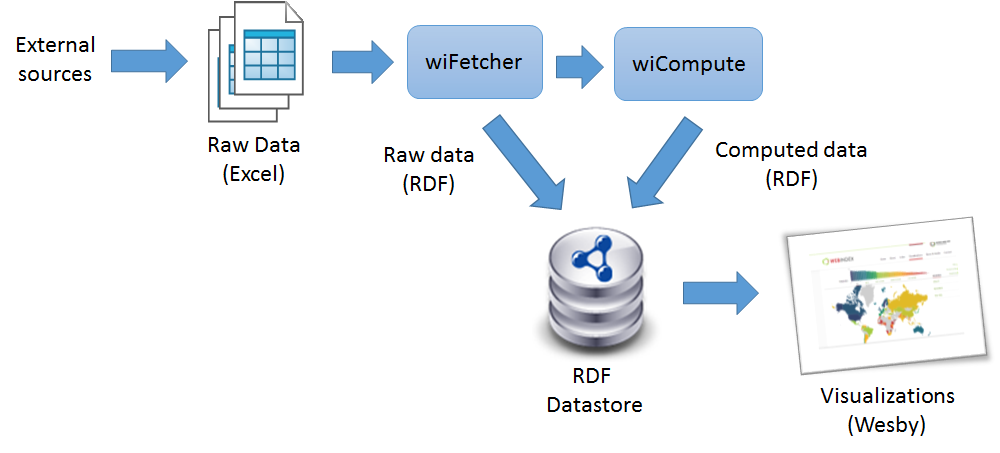
\includegraphics[width=\textwidth]{WebIndexFlow}
\end{center}
\caption{Web Index data portal WorkFlow}
\label{Fig:WebIndexWorkFlow}
\end{figure*}

The WebIndex workflow has been depicted in figure~\ref{Fig:WebIndexWorkFlow}. 
The Excel file was comprised of 184 Excel sheets and contained a combination
 of raw, imputed and normalized data created by the statistical experts. 

That external data was filtered and converted to RDF by means of an specialized web service called \emph{wiFetcher}\footnote{\url{https://github.com/weso/wiFetcher}}. 

Although some of the imported values had been
 pre-computed in Excel by human experts, we collected only the raw values, so we could automatically compute and validate the results. 

In this way, another application called \emph{wiCompute}\footnote{\url{https://github.com/weso/wiCompute}} 
 took the raw values and computed the index following the
 computation steps defined by the experts. 
\emph{wiCompute} carried out the computations
 generating RDF datasets for the intermediary results and linking the generated values
 to the values from which they had been computed.
 
Finally, the RDF data generated was published to a SPARQL endpoint from which we created
a specialized visualization tool called \emph{Wesby}\footnote{\url{https://github.com/weso/wesby}}.


\section{WebIndex data model}

Given the statistical nature of the data, the WebIndex data model is based on the RDF Data Cube vocabulary. Figure~\ref{Model} represents the main concepts of the data model

\begin{figure*}[h]
\label{Model}
\begin{center}
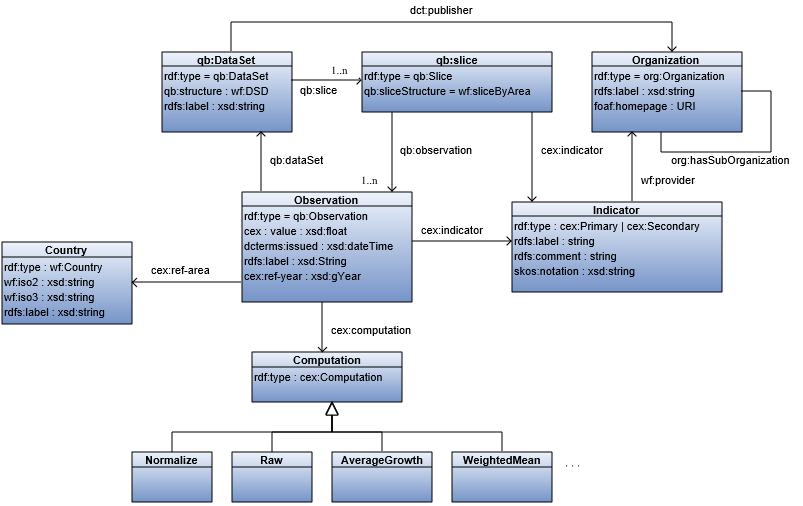
\includegraphics[width=\textwidth]{Model}
\end{center}
\caption{WebIndex data model}
\end{figure*}

As can be seen, the main concept are observations of type \lstinline|qb:Observation|, which 
can be raw observations,
obtained from an external source, 
or computed observations derived from other observations. 
Each observation has a float value \lstinline|cex:value| 
and is related to a country, a year, a dataset 
and an indicator.

A dataset contains a number of slices, each of which also contains a number of observations. 

Indicators are provided by an organization of type \lstinline|org:Organization| from the Organization ontology\cite{Organization14}. Datasets are also published by organizations. 

As a sample of some data, 
an observation can be that Italy has $-0.80$ as the normalized value using Z-Scores in 2007 for the indicator WEF\_L (\emph{Impact of ICT on organizational models}) provided by the World Economic Forum. 
This information can be represented in RDF using Turtle syntax as\footnote{The real observation is \url{http://data.webfoundation.org/webindex/v2013/observation/computed_2007_1386752461095_26549}. The real URIs also include an internal long number used to uniquely identify each entity}:

\begin{lstlisting}[style=SPARQL]
obs:computed_26549 a qb:Observation ;
 cex:indicator indicator:WEF_L ;
 qb:dataSet dataset:d_52 ;
 cex:value "-0.80"^^xsd:double ;
 cex:ref-area country:Italy ;
 cex:ref-year 2007 ;
 sdmx-concept:obsStatus cex:Normalized ;
 cex:computation computation:c26550
 ...other properties omitted for brevity
 .
\end{lstlisting}

Notice that the WebIndex data model contains data that is completely interrelated. Observations are linked to indicators, datasets and computations. Datasets contain also links to slices and slices have links to indicators and observations again. 
Both datasets and indicators are linked to the organizations that publish or provide them. 

The following example contains a sample of interrelated 
data for this domain. 
 
\begin{lstlisting}[style=SPARQL]
dataset:d_52 a qb:DataSet ;
 qb:structure wf:DSD ;
 qb:slice slice:computed_54 , slice:computed_55, ...
 ...
slice:computed_54 a qb:Slice ;
 qb:sliceStructure wf:sliceByArea ;
 qb:observation obs:computed_26549, obs:computed_26941, ... ;
 ...
indicator:WEF_L a cex:SecondaryIndicator ;
 rdfs:label "Impact of ICT on organizational models"@en ;
 wf:provider-link org:WEF ;
 ...
org:WEF a org:Organization ;
 rdfs:label "World Economic Forum" ;
 foaf:homepage <http://www.weforum.org/> 
 .
country:ITA a wf:Country ;
 wf:iso2 "IT" ; wf:iso2 "ITA" ;
 rdfs:label "Italy" .
...
computation:c26550 a cex:Normalize ;
 cex:slice slice:WEF_L2007-Imputed ;
 cex:stdDesv "0.75"^^xsd:double ;
 cex:mean "4.39"^^xsd:double ;
 cex:observation obs:obs29761 
 .
\end{lstlisting}

Computed observations and datasets contain a property \lstinline|cex:computation| that associate them to a node of type \lstinline|cex:Computation| which links the computed observation to the observations
from which it has been obtained. In the above example, the computation \lstinline|c26550| indicates that it is a normalization of the observation \lstinline|obs:obs29761| using the observations
in slice \lstinline|slice:WEF_L2007-Imputed| which has a standard deviation of $0.75$ and a mean of $4.39$. 
Including these declarations, an external agent can verify if the value of the observation has been well computed or if it has been tampered. We also noticed that these declarations had another positive effect to debug the computation process in the development phase of the data portal.


\section{Computex vocabulary}

The \emph{Computex}\footnote{\url{http://purl.org/weso/ontology/computex}} vocabulary defines terms related to the
computation of statistical index data and can be seen as a specialization of the RDF Data Cube
vocabulary for this kind of statistical computations. Some terms defined in the vocabulary are:

\begin{itemize}
\item\textbf{\lstinline|cex:Concept|} represents the entities that we are
indexing.
In the case of the Web Index project, the concepts are the different countries.
In other applications it could be Universities, journals, services, etc.

\item\textbf{\lstinline|cex:Indicator|}. A dimension whose values add
information to the Index.
Indicators can be simple dimensions, for example: the mobile phone
suscriptions per 100 population, or can be composed from other
indicators. 

\item\textbf{\lstinline|cex:Computation|}. It represents a computation. We included the main computation types that we needed for the WebIndex project, which have been summarized in
Table~\ref{table:computations}. That list of computation types is non-exhaustive
and can be further extended in the future. 

\item\textbf{\lstinline|cex:WeightSchema|} a weight schema for a list of
indicators. It consists of a weight associated for each indicator which can be
used to compute an aggregated observation.

\end{itemize}

\begin{savenotes}
\begin{table*}[t]
\begin{center}
\begin{tabular}{ p{0.2\textwidth} p{0.5\textwidth} p{0.3\textwidth}}
\toprule
Computation & Description & Properties \\
\hline
Raw			& No computation. Raw value obtained from external source.
			&  \\
Mean	    & Mean of a set of observations 
			& \lstinline|cex:observation| \newline 
			  \lstinline|cex:slice| \\
Increment	& Increment an observation by a given amount 
			& \lstinline|cex:observation| \newline 
			  \lstinline|cex:amount|  \\
Copy		& A copy of another observation 
			& \lstinline|cex:observation| \\
Z-score		& A normalization of an observation using the values from a Slice. 
			& \lstinline|cex:observation| \newline 
			  \lstinline|cex:slice| \\
Ranking		& Position in the ranking of a slice of observations. 
			& \lstinline|cex:observation| \newline 
			  \lstinline|cex:slice| \\
AverageGrowth & Expected average growth of N observations
			  & \lstinline|cex:observations|\footnote{This is in plural because the value of this property is an ordered list of observations} \\
WeightedMean & Weighted mean of an observation
			& \lstinline|cex:observation| \newline
			  \lstinline|cex:slice|       \newline
			  \lstinline|cex:weightSchema| \\
\bottomrule\\
\end{tabular}
\end{center}
\caption{Some types of statistical computations}\label{table:computations}
\end{table*}
 \end{savenotes}
\section{Development and Validation approach}

The validation approach employed in the 2012 WebIndex project was based on ad-hoc resource templates and a MD5 checksum field. 
 Apart from that, we did not verify that the precomputed values imported from
 the Excel sheets really matched the value that could be obtained by 
 following the declared computation process.

In the 2013 version, we did a step forward on the validation approach. 
The goal was not only to check that a resource contained a given set of fields and values, but also that those values really matched
the values that can be obtained by following the declared computations.
 
The proposed approach was inspired by the integrity constraint specification proposed by the RDF Data Cube vocabulary, 
which employs a set of SPARQL
 \lstinline|ASK| queries to check the integrity of RDF Data Cube data. 
 Although \lstinline|ASK| queries provide a good means to check integrity, in
 practice their boolean nature does not offer too much help when a 
 dataset does not accomplish with the data model.

We decided to use \lstinline|CONSTRUCT| queries which, in case of error, 
  contain an error message and a list of error parameters that can help to spot
  the problematic data.

 We transformed the \lstinline|ASK| queries defined in the RDF Data Cube
 specification to \lstinline|CONSTRUCT| queries. 
In order to make our error messages compatible with EARL~\cite{EARL}, we have
 defined \lstinline|cex:Error| as a subclass of \lstinline|earl:TestResult| and 
 declared it to have the value \lstinline|earl:failed| for the property
 \lstinline|earl:outcome|.
 
We have also created our own set of SPARQL \lstinline|CONSTRUCT| queries to
validate the \emph{Computex} vocabulary terms, specially the computation of index data.
For example, the following query validates whether every observation 
  has at most one value.
 
\begin{lstlisting}[style=SPARQL]
CONSTRUCT { [ a cex:Error ; cex:errorParam  # ... omitted 
              cex:msg "Observation has two different values" . ]
} WHERE { ?obs a qb:Observation . 
 ?obs cex:value ?value1 . ?obs cex:value ?value2 .
 FILTER ( ?value1 != ?value2  ) }
\end{lstlisting}

Using this approach, it is possible to define more expressive validations.
For example, we are able to validate whether an observation has been obtained as
the mean of other observations. 

\begin{lstlisting}[style=SPARQL]
CONSTRUCT { [ a cex:Error ; cex:errorParam # ...omitted 
   cex:msg "Mean value does not match" ] . 
} WHERE { ?obs a qb:Observation ;
          cex:computation ?comp ;
          cex:value ?val .
          ?comp a cex:Mean .
   { SELECT (AVG(?value) as ?mean) ?comp WHERE {
     ?comp cex:observation ?obs1 .
	 ?obs1 cex:value ?value ;
     } GROUP BY ?comp } 
 FILTER( abs(?mean - ?val) > 0.0001) }
\end{lstlisting}

Validating statistical computations using SPARQL queries offered 
 a good exercise to check SPARQL expressiveness. Although we were able 
 to express most of the computation types, some of them had to employ functions
 that were not part of SPARQL 1.1 or had to be defined in a limited way. We described these limits in~\cite{Labra13}.

We implemented an online validation tool called \emph{Computex}\footnote{\url{http://computex.herokuapp.com/}} which takes as
 input an RDF graph and checks if it follows the integrity constraints defined by Computex.
 The validation tool can also check if the RDF graph follows the RDF Data Cube integrity constraints
 and it can also do the index computation for RDF Graphs. 
 Although this declarative approach was very elegant, computing the webindex using only SPARQL queries
 was not practical (it took around 15 minutes for a small subset), so the computation process was finally done
 by a specialized program implemented in Scala~\footnote{Source code is available here: \url{https://github.com/weso/wiCompute}}. 
  
\section{Visualizing the data portal}

We developed a visualization tool called Wesby~\footnote{\url{http://wesby.weso.es}} which takes as input an SPARQL endpoint and offers a linked data browsing experience. Wesby was inspired by Pubby~\cite{Pubby} and was developed in Scala using the Play! Framework. 
Wesby combines the visualization with a set of templates to offer specialized views for different types of resources. For example, figure~\ref{Fig:WebIndexItaly} contains the WebIndex visualization of 
 Italy\footnote{It can be seen here: \url{http://data.webfoundation.org/webindex/v2013/country/ITA}}. The interactive visualization graphics use a javascript library called WesCountry that we have also developed~\footnoteUrl{http://weso.github.io/wesCountry/}.

\begin{figure*}[h]
\begin{center}
  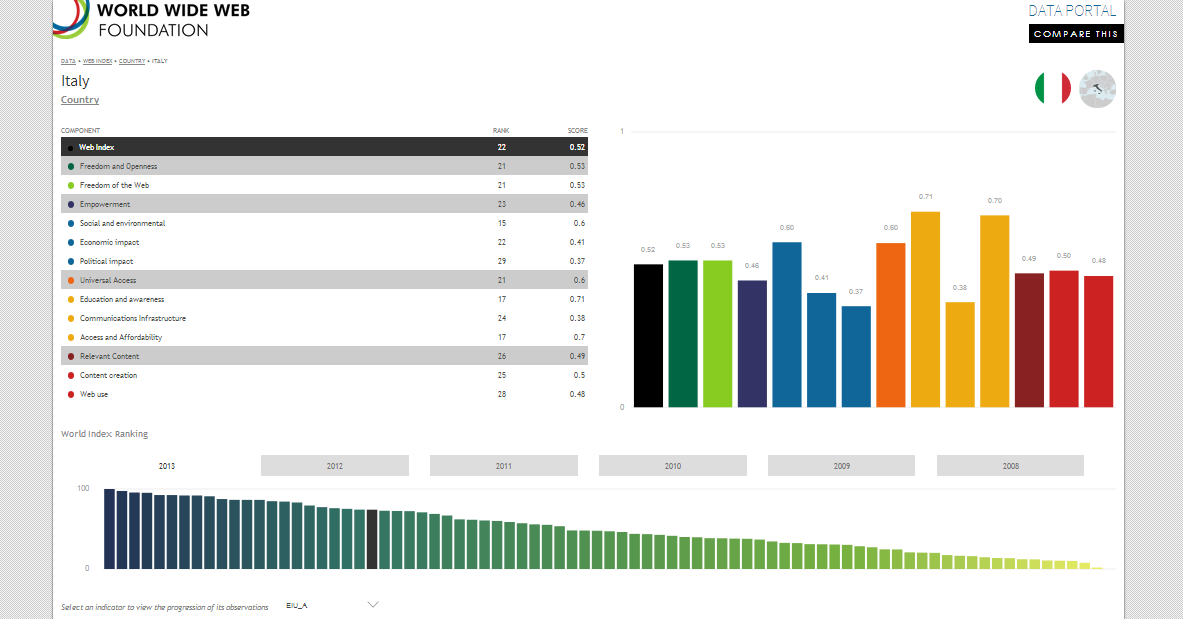
\includegraphics[width=\textwidth]{WebIndexIta}
\end{center}
\caption{Web Index visualization of country Italy}
\label{Fig:WebIndexItaly}
\end{figure*}

When there is no template for a given type of node, Wesby shows a table of properties and values similar to Pubby. Wesby also handles content negotiation so it can return different representations depending on the \lstinline|ACCEPT| header.

In order to document the resulting data portal we created a set of templates using Shape Expressions~\footnote{\url{http://weso.github.io/wiDoc/}}. We consider that this approach offers a good balance between human readability and machine processable specification. 
  
\section{Related work}

There is a growing interest in developing solutions to improve the quality of linked data~\cite{hogan10,Mendes12,kontokostasDatabugger}. 
We consider that it is very important to publish linked data that is not only of high
 quality, but also that can automatically be validated. 
 Validating RDF has also attracted a number of approaches. 
 Most of them were presented at the W3c Workshop on RDF Validation~\cite{RDFValidation} and can
be classified as inference based, SPARQL queries or grammar based.

Inference based approaches try to adapt
OWL for validation proposes. 
However, the use of Open World and Non-unique name assumption limits the
validation possibilities. 
A variation of OWL semantics using Closed World Assumption to express integrity constraints has been proposed in \cite{ClarkSirin13,Tiao10,Motik07}.
SPARQL queries can also express validation constraints and offer a great level of expressiveness~\cite{Labra13}. 
Grammar based approaches like OSLC Resource Shapes~\cite{OSLCResourceShapes} and Dublic Core Application Profiles~\cite{KarenCoyleTomBaker13} define a domain specific language to declare the validation rules. Recently, Shape Expressions~\cite{Boneva2014} have been proposed as a new technology to describe and validate RDF data portals. 

Representing statistical linked data has also seen an increasing interest. 
SDMX~\footnote{\url{http://sdmx.org/}} is the primary format of the main statistical data organizations. The transformation of SDMX-ML to RDF/XML has been described in~\cite{Capadisli13}.
The RDF Data Cube vocabulary~\cite{Cube} has been accepted as a W3c Recommendation technology to publish multi-dimensional statistical data and to link it with other concepts and data. 
We have opted to follow the RDF Data Cube vocabulary and in fact, we consider that Computex can be seen as a further specialization of RDF Data Cube to represent statistical index computations.

Another line of related work is the representation of mathematical expressions as linked data. 
Lange~\cite{Lange13} gives an overview of the different approaches. 
OpenMath was proposed as an extensible standard that can represent the semantic meaning of mathematical objects. 
Wenzel and Reinhardt~\cite{Wenzel12} 
propose an approach to integrate OpenMath with
RDF data for the representation of mathematical relationships and the integration
of mathematical computations into reasoning systems.
We consider \emph{Computex} as a first step in that 
direction to represent statistical computations and 
we expect more future work to appear about how to
represent statistical computations as linked data.

\section{Conclusions}

In this paper, we described how we were able to represent statistical index computations as linked data which include information to track the origin of any published observation. 
Although the number of triples were around 3,5 million, we consider that the data portal is of medium size, so we were able to play with different validation possibilities.

Although we have been able to express most of the computations using SPARQL queries, we have found some
limitations in current SPARQL 1.1 expressiveness with regards to built-in
functions on maths, strings, RDF Collections and performance. In fact, although we initially wanted to do the whole computation process using SPARQL CONSTRUCT queries, we found that it took longer than expected and was difficult to debug, so we opted to develop an independent program that did all the computation process in a few seconds.

After participating in the W3c RDF Validation workshop we were attracted by the Shape Expressions formalism so we developed the documentation of the WebIndex data portal using Shape Expressions. We consider that some structural parts of the data portal can be better expressed in Shape Expressions.

Our future work is to automate the declarative computation of index data
 from the raw observations and to check the performance using
 the Web Index data. We are also improving the Wesby visualization tool and the WesCountry library for statistical graphics. We are even considering to relate visualization templates with Shape Expressions offering a better separation of concerns in the development process.

% \TODO{Visualization of computed values?}

\section{Acknowledgements}

We would like to thank Jules Clements, Karin Alexander, César Luis Alvargonzález, Ignacio Fuertes Bernardo and Alejandro Montes for their collaboration in the development of the WebIndex project.

\bibliographystyle{abbrv}
\bibliography{computex}

\end{document}
